\documentclass{beamer}

%% \documentclass[handout]{beamer}
%% % use this with the [handout] option to create handouts for the audience
%% \usepackage{pgfpages}
%% \pgfpagesuselayout{2 on 1}[a4paper,border shrink=5mm]

\mode<presentation>
{
  \usetheme{Diku}
% set this to your preferences:
  \setbeamercovered{invisible}
%  \setbeamercovered{transparent}
}

\usepackage{graphicx}
\usepackage{epic}

\usepackage{amsmath}
\usepackage{amssymb}
\usepackage{amsthm}

\usepackage{minibox}

\newcommand{\basetop}[1]{\vtop{\vskip-1ex\hbox{#1}}}
\newcommand{\source}[1]{\let\thefootnote\relax\footnotetext{\scriptsize\textcolor{kugray1}{Source: #1}}}

% for coloured code citation in text:
\usepackage{fancyvrb}

%%%%%%%%%%%%%%%%%%%%%%%%%%%%%%%%%
%%%%%    code sections   %%%%%%%%
%%%%%%%%%%%%%%%%%%%%%%%%%%%%%%%%%

% code highlighting commands in own block
\DefineVerbatimEnvironment{code}{Verbatim}{fontsize=\scriptsize}
\DefineVerbatimEnvironment{icode}{Verbatim}{fontsize=\scriptsize}

% Fancy code with color commands:
\DefineVerbatimEnvironment{colorcode}%
        {Verbatim}{fontsize=\scriptsize,commandchars=\\\{\}}

%%%%%%%%%%%%%%%%%%%%%%%%%%%%%%%%%%
%%%%%    some coloring    %%%%%%%%

\definecolor{Red}{RGB}{220,50,10}
\definecolor{Blue}{RGB}{0,51,102}
\definecolor{Yellow}{RGB}{102,51,0}
\definecolor{Orange}{RGB}{178,36,36}
\definecolor{Grey}{RGB}{180,180,180}
\definecolor{Green}{RGB}{20,120,20}
\definecolor{Purple}{RGB}{160,50,100}
\newcommand{\red}[1]{\textcolor{Red}{{#1}}}
\newcommand{\blue}[1]{\textcolor{Blue}{{#1}}}
\newcommand{\yellow}[1]{\textcolor{Yellow}{{#1}}}
\newcommand{\orange}[1]{\textcolor{Orange}{{#1}}}
\newcommand{\grey}[1]{\textcolor{Grey}{{#1}}}
\newcommand{\green}[1]{\textcolor{Green}{{#1}}}
\newcommand{\purple}[1]{\textcolor{Purple}{{#1}}}




% use "DIKU green" from our color theme for \emph
\renewcommand{\emph}[1]{\textcolor{structure}{#1}}
% use some not-too-bright red for an \emp command
\definecolor{DikuRed}{RGB}{130,50,32}
\newcommand{\emp}[1]{\textcolor{DikuRed}{ #1}}
\definecolor{CosGreen}{RGB}{10,100,70}
\newcommand{\emphh}[1]{\textcolor{CosGreen}{ #1}}
\definecolor{CosBlue}{RGB}{55,111,122}
\newcommand{\emphb}[1]{\textcolor{CosBlue}{ #1}}
\definecolor{CosRed}{RGB}{253,1,1}
\newcommand{\empr}[1]{\textcolor{CosRed}{ #1}}

\newcommand{\mymath}[1]{$ #1 $}
\newcommand{\myindx}[1]{_{#1}}
\newcommand{\myindu}[1]{^{#1}}

\newcommand{\Fasto}{\textsc{Fasto}\xspace}


%%%%%%%%%%%%%%%%%%%%

\title[TAC Optim.]{Three-Address-Code (TAC) Optimizations}

\author[C.~Oancea]{Cosmin E. Oancea\\{\tt cosmin.oancea@diku.dk}}

\institute{Department of Computer Science (DIKU)\\University of Copenhagen}


\date[December 2012]{December 2012 Compiler Lecture Notes}


\begin{document}

\titleslide

\input{Struct_Interm/StructTACoptim}

\begin{frame}[fragile]
	\tableofcontents
\end{frame}


%%%%%%%%%%%%%%%%%%%%%%%%%%%%%%%%%%%%%%%%%%%%%%%%%%%%%%%%%%%%%%%%%%%%%%
%%%%%%%%%%%%%%%%%%%%%%%%%%%%%%%%%%%%%%%%%%%%%%%%%%%%%%%%%%%%%%%%%%%%%%
\section{Optimizations: Bird-Eye View}

\begin{frame}\frametitle{Code-Optimization Motivation and Requirements}

Compiler's target code is still \emp{not as good} as the hand-tuned code of
the assembly-language \emp{expert}, but is \emph{better} than what \emph{most
programmers} would generate, even if they wanted to.

\bigskip

Achieved via code transformations, albeit the result is hardly optimal.

\bigskip
\pause

\emp{An optimization}, a.k.a., code transformation, \emp{needs to}:


\begin{itemize}

\item \alert{preserve the observable behavior of the original prg (semantics),}\smallskip

\item speed-up the program by a measurable amount (on average),\smallskip

\item prg's size not an issue but may affect instr-cache performance,\smallskip

\item be worth the effort, e.g., compile time, maintainability, etc.

\end{itemize}

\end{frame}



\begin{frame}\frametitle{High-Level Optimization Strategy}

The compiler effort for a certain code fragment is relative to:

\smallskip

\begin{itemize}

\item the number of times the prg will be run (user sets optim level);\smallskip

\item the amount of time spent in that code fragment relative to the
        progrm's runtime.\smallskip

\end{itemize}

\pause
\bigskip

Code optimization problems are NP-complete or undecidable:

\smallskip

\begin{itemize}

\item in many cases even NP-complete to aproximate, hence\smallskip

\item cannot expect to find a global optimum in a reasonable time.\smallskip

\end{itemize}

\pause
\bigskip

Strategy: spend the compiler effort in hot areas, e.g., loop nests:

\begin{itemize}

\item programers can write clear code in high-level languages\smallskip

\item while still getting efficient execution.\smallskip

\end{itemize}

\end{frame}



\begin{frame}\frametitle{Optimization Break Down}

\minibox{Source\\Code}{\tt~~}\blue{$\Rightarrow$}{\tt~~}\framebox{\minibox{Front\\End}}{\tt~~}\blue{$\Rightarrow$}{\tt~~}\minibox{Interm\\Code}{\tt~~}\blue{$\Rightarrow$}{\tt~~}\framebox{\minibox{Code\\Generator}}{\tt~~}\blue{$\Rightarrow$}{\tt~~}\minibox{Target\\Code}

\bigskip
\bigskip

\begin{tabular}{lll}
\green{User can:} & \emp{Compiler Can}: & \emp{Compiler Can}:\\
& & \\
profile program & improve loops & use register\\
change algorithm & re-order/pipeline loops & select/reorder instrs\\
transform loops & optimize procedure calls & peephole transfs\\
 & eliminate procedure calls & \\
 & straighten code & \\
 & recognize common subexps & \\
 & compute constant subexps & \\
 & propagate constants  & \\
 & ... and lots more  & 
\end{tabular}

\end{frame}


%%%%%%%%%%%%%%%%%%%%%%%%%%%%%%%%%%%%%%%%%%%%%%%%%%%%%%%%%%%%%%%%%%%%%%
%%%%%%%%%%%%%%%%%%%%%%%%%%%%%%%%%%%%%%%%%%%%%%%%%%%%%%%%%%%%%%%%%%%%%%
\section{Recovering Program Structure from TAC}

\begin{frame}[fragile]
	\tableofcontents[currentsection]
\end{frame}

%%%%%%%%%%%%%%%%%%%%%%%%%%%%%%%%%%%%%%%%%%%%%%%%%%%%%%%%%%%%%%%%%%%%%%
\subsection{Basic Blocks}



\begin{frame}[fragile,t]
    \frametitle{Optimizations at Three-Address-Code (TAC) Level}

Interm-lang optimizations, e.g., \textsc{TAC}, portable to various backends:

\smallskip

\begin{itemize}

\item \textsc{TAC} is more flexible than \textsc{AbSyn} for local code transformations,\smallskip

\item \emph{we can rebuild the control-flow or global structure from \textsc{TAC}!}\smallskip

\end{itemize}

\pause
\bigskip

\emp{A basic block} is a \textsc{TAC} sequence where the flow of control 
enters at the begining and leaves at the end:

\smallskip

\begin{block}{Example of a Basic Block (straight-line code):}
\begin{colorcode}[fontsize=\scriptsize]
\blue{L3:} t5 := a  * b
    t6 := t5 + c
    d  := t2 * t2
    \emp{if(d = 0) goto L4}
\end{colorcode} 
\end{block}


\bigskip

Local Optimizations: reordering \textsc{TAC} instructions in a basic block.\smallskip
Need to \emp{worry about the effects} caused to the values of the variables
at the \emp{start/end of the block}.

\end{frame}




\begin{frame}[fragile,t]
    \frametitle{Identifying Basic Blocks (BB)}


\begin{itemize}

\item Find the statements that \blue{start a basic block (BB)}:\smallskip
    \begin{itemize}
        \item first statement of any function

        \item any labeled statement that is the target of a branch

        \item any statement following a branch (conditional or unconditional)\smallskip
    \end{itemize}


\item \blue{for each statement starting a BB, the BB consists of all stmts up
            to, but excluding, the start of a BB or the end of the program!}

\end{itemize}

\bigskip

\begin{block}{Example: Finding Basic Blocks and The Control-Flow Graph (\textsc{CFG})}
\begin{colorcode}[fontsize=\scriptsize]
    i := 20
    s := 0
L1:
    if i=0 \emp{goto L2}
    s := s + i
    i := i - 1
    \emp{goto L1}
L2:
\end{colorcode} 
\end{block}

\end{frame}


%%%%%%%%%%%%%%%%%%%%%%%%%%%%%%%%%%%%%%%%%%%%%%%%%%%%%%%%%%%%%%%%%%%%%%%%%%%%%%%%%%%%
\subsection{Control-Flow Graph (CFG)}


\begin{frame}[fragile,t]
    \frametitle{Control-Flow Graph (CFG)}


\begin{itemize}

\item Find the statements that \blue{start a basic block (BB)}:\smallskip
    \begin{itemize}
        \item first statement of any function

        \item any labeled statement that is the target of a branch

        \item any statement following a branch (conditional or unconditional)\smallskip
    \end{itemize}


\item \blue{for each statement starting a BB, the BB consists of all stmts up
            to, but excluding, the start of a BB or the end of the program!}

\end{itemize}

\bigskip

\begin{block}{Example: Finding Basic Blocks and The Control-Flow Graph (\textsc{CFG})}
\begin{columns}
\column{0.18\textwidth}
\begin{colorcode}[fontsize=\scriptsize]
    \blue{i := 20}
    s := 0
\blue{L1:}
    if i=0 \emp{goto L2}
    \blue{s := s + i}
    i := i - 1
    \emp{goto L1}
\blue{L2:}
\end{colorcode} 
\column{0.4\textwidth}
\includegraphics[width=25ex]{Figures/CFGeg1}
\column{0.33\textwidth}
\emp{Control-Flow Graph:}\\
BBs are nodes in CFG.\\
{\tt~}\\
Place an arrow from
node $A$ to node $B$ if it is
possible for control to
``flow'' from $A$ to $B$.
\end{columns}
\end{block}

\end{frame}



%%%%%%%%%%%%%%%%%%%%%%%%%%%%%%%%%%%%%%%%%%%%%%%%%%%%%%%%%%%%%%%%%%%%%%
\subsection{Identifying Loops}


\begin{frame}[fragile,t]
    \frametitle{Identifying Loops, Preliminaries}

{\bf Motivation}: loops is where most of the time is spend!

\pause
\bigskip

{\bf Defition}: A loop, $L$, is a subgraph of the \textsc{CFG} such that:

\begin{itemize}

\item all nodes of the loop are \emp{strongly connected}, i.e., the loop
        contains a path between any two loop nodes.

\item the loop has \green{an unique entry point}, named \emph{header}, such that

\item the only way to reach a loop node is through the entry point.

\end{itemize}

A loop that contains no other loop is called an {\em inner loop}.

\pause
\bigskip

{\bf Dominator Definition}: a node $p$ \emp{dominates} node $q$ if all paths from
the start of the program to $q$ go through $p$.

\bigskip

{\bf Identifying} loops requires finding their ``\emp{back edges}'':

\begin{itemize}

\item edges in the program in which the destination node dominates
        the source node.

\item a loop must have \green{an unique header}, and \emp{one or more backedges}.

\item header dominates all blocks in the loop, otherwise not unique.

\end{itemize}

\end{frame}





\begin{frame}[fragile,t]
    \frametitle{Example of a Loop CFG}

\bigskip

\begin{block}{Example: Finding Basic Blocks and The Control-Flow Graph (CFG)}
\begin{columns}
\column{0.3\textwidth}
\begin{colorcode}[fontsize=\scriptsize]
    s := 0
    i := 0
    n := 10
\blue{L1:}
    t1 := a - b
    if t1 = 0 \emp{goto L2}
    t2 := i * 4
    s := s + t2
    \emp{goto L3}
\blue{L2:} s := s + i
\blue{L3:} i := i + 1
    t3 := n - i
    if t3 != 0 \emp{goto L1}
    t4 := a - b
    CALL PRINT(t4)
\end{colorcode} 
\column{0.6\textwidth}
\includegraphics[width=33ex]{Figures/LoopEg}
\end{columns}
\end{block}

\end{frame}





\begin{frame}[fragile,t]
    \frametitle{Identifying Loops}

\bigskip

\begin{block}{Algorithm for Dominators. $D(n)$ is the set of dominators of block $n$.}
%\begin{colorcode}[fontsize=\scriptsize]
{\bf Input}: \textsc{CFG} with node set $N$, initial node $n_0$.
{\bf Output}: $D(n), \forall n \in N$\\
$D(n_0) := \{ n_0 \}$\\
for $n \in N - \{n_0\}$ do $D(n)$ := $N$\\
{\tt~~}\\
while changes to any $D(n)$ occur do\\
{\tt~~~~}for $n \in N - \{n_0\}$ do\\
{\tt~~~~~~~~}$D(n)$ := $\{n\} \cup \alert{(\cap_{p\in pred(n)} D(p))}$
%\end{colorcode} 
\end{block}

\pause
\bigskip

{\bf High-Level Algorithm}: With each \emp{backedge $n \rightarrow d$}
($d$ is the loop header), we associate a \green{natural loop} (of $n \rightarrow d$) 
consisting of node $d$ and all nodes that can reach $n$ without going through $d$.

\bigskip

{\bf Intuition}: since $d$ is the only entry to the loop, a path from any
block outside the loop must pass through $d$.

\end{frame}


%%%%%%%%%%%%%%%%%%%%%%%%%%%%%%%%%%%%%%%%%%%%%%%%%%%%%%%%%%%%%%%%%%%%%%
\subsection{Control-Flow-Graph Reducibility}

\begin{frame}[fragile,t]
    \frametitle{Reducible Control-Flow Graphs}

\begin{block}{Which one is the innermost?{\tt~~~~~~~}Improper Loop}
\begin{columns}
\column{0.3\textwidth}
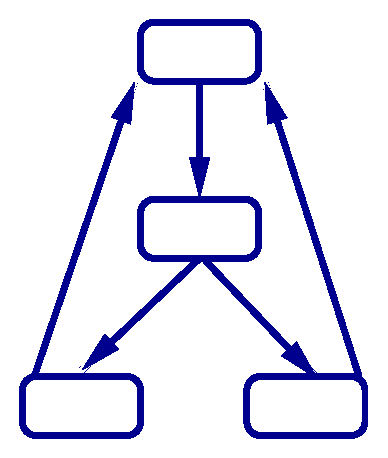
\includegraphics[width=17ex]{Figures/LoopAwk}
\column{0.6\textwidth}
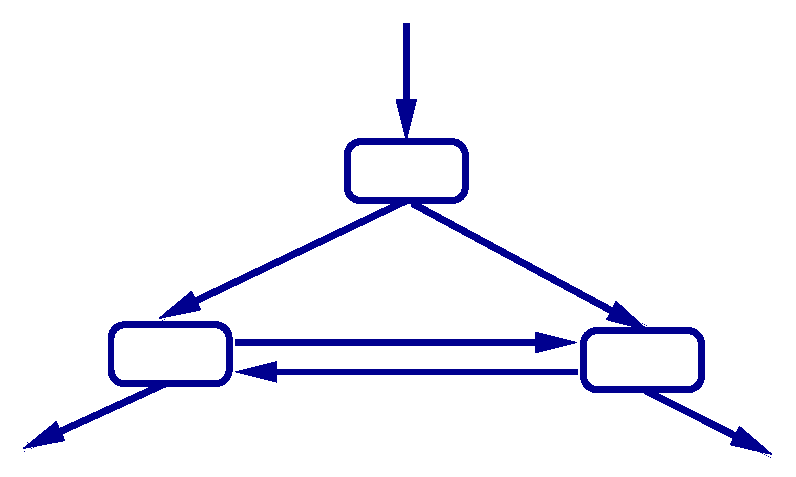
\includegraphics[width=34ex]{Figures/LoopUnstruct}
\end{columns}
\end{block}

{\bf A CFG is reducible} if it can be partitioned in forward and backward
edges, where the forward edges form a directed-acyclic graph.\smallskip

Non-reducible CFG: from unstructured use of GOTO \& from allowing jumps
into loops from outside the loop.

\bigskip

{\bf Key property}: if a CFG is reducible then all cycles are (regular)
loops, and identifying the backedges is enough to find all loops.

\end{frame}




\begin{frame}[fragile,t]
    \frametitle{Testing and Solving Ireducible CFG}

\bigskip

\begin{block}{Alg for Testing Reducibility{\tt~~~~~~~~~~}Node Splitting}
\begin{columns}
\column{0.41\textwidth}
In a copy of the \textsc{CFG}, apply\\
{\tt T1} and {\tt T2} to a fixpoint. If\\
the result is a single node\\
than the \textsc{CFG} is reducible.\\
%
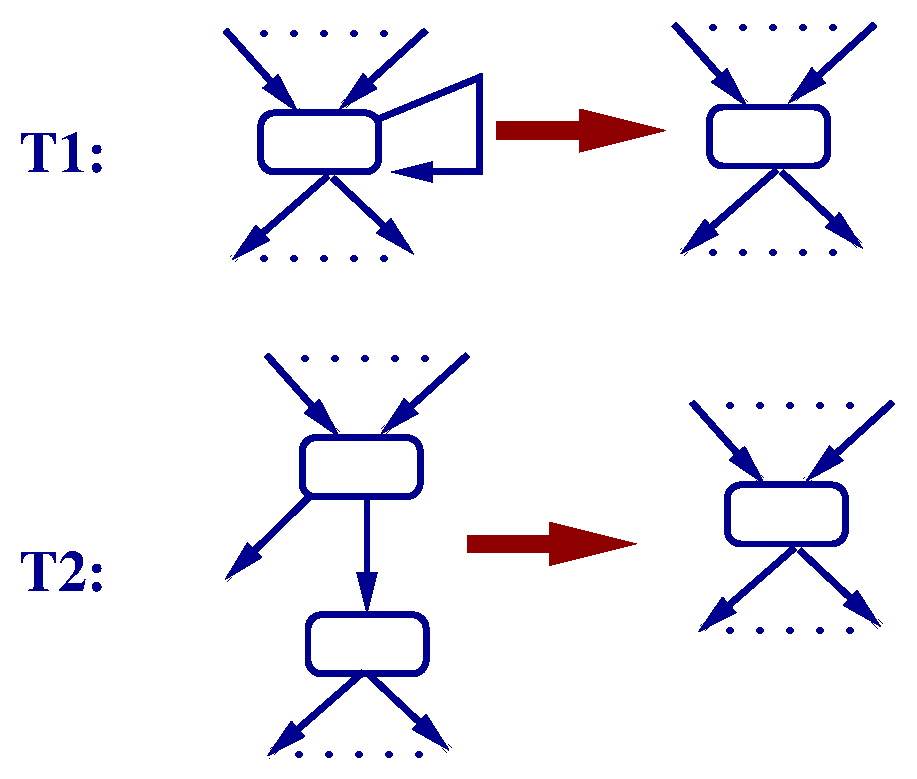
\includegraphics[width=17ex]{Figures/T12}
\column{0.55\textwidth}
Irreducible \textsc{CFG}s are difficult to\\
optimize. It is always possible to solve\\
irreducibility, but, in the worst case, at\\
the cost of an exponential-code explosion:\\
%
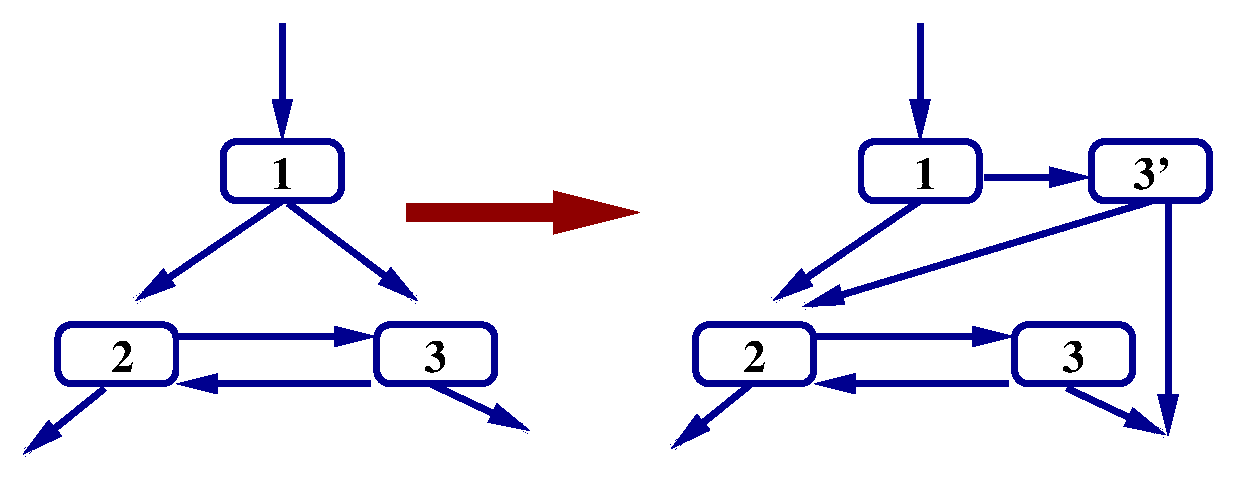
\includegraphics[width=34ex]{Figures/NodeSplit}
\end{columns}
\end{block}

\end{frame}


%%%%%%%%%%%%%%%%%%%%%%%%%%%%%%%%%%%%%%%%%%%%%%%%%%%%%%%%%%%%%%%%%%%%%%
%%%%%%%%%%%%%%%%%%%%%%%%%%%%%%%%%%%%%%%%%%%%%%%%%%%%%%%%%%%%%%%%%%%%%%
\section{Examples of Optimizations}

\begin{frame}[fragile]
	\tableofcontents[currentsection]
\end{frame}


\begin{frame}[fragile,t]
    \frametitle{Example of Optimizations}

We have already seen \emp{\bf liveness analysis \& register allocation}.

\bigskip

\emp{\bf Common-Subexpression Elimination (CSE)}: if the same expression
$e$ is computed twice, replace if possible the second occurrence of $e$
with the temporary that holds the value of the first computation of $e$.

\bigskip

\emp{\bf Copy Propagation (CP)}: after a statement {\tt x~:=~y}, 
we know that {\tt x} and {\tt y} have the same value, hence we can replace 
all occurrences of {\tt x} with {\tt y} between this assignment and the next 
definition of {\tt x} or {\tt y}.

\bigskip

\emp{\bf Dead-Code Elimination (DC)} (one reason is copy propagation):
\begin{itemize}
    \item can safely remove any statement that defines a dead variable,
    \item a branch to dead code moved to whatever follows the dead code,
    \item if a branch-condition value is statically known $\Leftrightarrow$ merge two BBs.
\end{itemize}

\bigskip

\emp{\bf Constant Folding and Propagation (CtF/P)}: if possible,
expressions should be computed at compile time, and the constant
result should be propagated. {\bf And these are just a few!}


\end{frame}




\begin{frame}[fragile,t]
    \frametitle{Example: Common-Subexpression Elimination
                    (CSE) and Copy Propagation (CP)}

\bigskip

\begin{block}{Original{\tt~~~~~~~}After CSE1{\tt~~~~~~}After CP1{\tt~~~}After CSE2 \& CP2}
\begin{columns}
\column{0.18\textwidth}
\begin{colorcode}[fontsize=\scriptsize]
t1 := 4  - 2
t2 := t1 / 2
t3 := a  * t2
t4 := \emp{t3 * t1}
t5 := t4 + b
t6 := \emp{t3 * t1}
t7 := t6 + b
c  := t5 * t7
\end{colorcode} 
\column{0.22\textwidth}
\begin{colorcode}[fontsize=\scriptsize]
t1 := 4  - 2
t2 := t1 / 2
t3 := a  * t2
t4 := t3 * t1
t5 := t4 + b
\emp{t6} := \green{t4}
t7 := \emp{t6} + b
c  := t5 * t7
\end{colorcode} 
\column{0.22\textwidth}
\begin{colorcode}[fontsize=\scriptsize]
t1 := 4  - 2
t2 := t1 / 2
t3 := a  * t2
t4 := t3 * t1
\green{t5} := \emp{t4 + b}
t6 := t4
t7 := \emp{t4 + b}
c  := t5 * t7
\end{colorcode} 
\column{0.22\textwidth}
\begin{colorcode}[fontsize=\scriptsize]
t1 := 4  - 2
t2 := t1 / 2
t3 := a  * t2
t4 := t3 * t1
t5 := \emp{t4 + b}
t6 := t4
t7 := t5
c  := t5 * \green{t5}
\end{colorcode} 
\end{columns}
\end{block}

\bigskip

Copy propagation makes further common-subexpression elimination
possible and the reverse.

\end{frame}





\begin{frame}[fragile,t]
    \frametitle{Example Continuation: Constant Folding (CFP) \&
                    Copy Propagation (CP) \& Dead Code Elim (DCE)}

\bigskip

\begin{block}{Original{\tt~~~~~~}After CtFP{\tt~~~~~~~}After CP{\tt~~~~~~~~}After DCE}
\begin{columns}
\column{0.18\textwidth}
\begin{colorcode}[fontsize=\scriptsize]
\emp{t1 := 4  - 2}
\emp{t2 := t1 / 2}
t3 := a  * \emp{t2}
t4 := t3 * \emp{t1}
t5 := t4 + b
t6 := t4
t7 := t5
c  := t5 * t5
\end{colorcode} 
\column{0.22\textwidth}
\begin{colorcode}[fontsize=\scriptsize]
t1 := 2
t2 := 1
\emp{t3 := a}
t4 := \emp{t3} * 2
t5 := t4 + b
t6 := t4
t7 := t5
c  := t5 * t5
\end{colorcode} 
\column{0.22\textwidth}
\begin{colorcode}[fontsize=\scriptsize]
\emp{t1 := 2}
\emp{t2 := 1}
\emp{t3 := a}
t4 := a  * 2
t5 := t4 + b
\emp{t6 := t4}
\emp{t7 := t5}
c  := t5 * t5
\end{colorcode} 
\column{0.22\textwidth}
\begin{colorcode}[fontsize=\scriptsize]



t4 := a  * 2
t5 := t4 + b


c  := t5 * t5
\end{colorcode} 
\end{columns}
\end{block}

\bigskip

One of the main difficulties is deciding in which order to apply 
these optimizations, and how many times to apply them...

\end{frame}


%%%%%%%%%%%%%%%%%%%%%%%%%%%%%%%%%%%%%%%%%%%%%%%%%%%%%%%%%%%%%%%%%%%%%%
%%%%%%%%%%%%%%%%%%%%%%%%%%%%%%%%%%%%%%%%%%%%%%%%%%%%%%%%%%%%%%%%%%%%%%
\section{Data-Flow Analysis}

\begin{frame}[fragile]
	\tableofcontents[currentsection]
\end{frame}

\begin{frame}[fragile,t]
    \frametitle{Data-Flow Analysis}

Global analysis is used to derive information that can drive
optimizations. Example: {\em Liveness analysis.}


\bigskip

Information can flow forwards or backwards through the program.\\
Typical Structure:\smallskip

\begin{itemize}
    \item Successor/predecessor on basic blocks ($succ[B_i]$ or $pred[B_i]$).\smallskip
    \item Define $gen[i]$ and $kill[i]$ sets.\smallskip
    \item Define equations for $in[i]$ and $out[i]$.\smallskip
    \item Initialize $in[i]$ and $out[i]$.\smallskip
    \item Iterate to a fix point.\smallskip
    \item Use $in[i]$ or $out[i]$ for optimizations.
\end{itemize}

\end{frame}


%%%%%%%%%%%%%%%%%%%%%%%%%%%%%%%%%%%%%%%%%%%%%%%%%%%%%%%%%%%%%%%%%%%%%%
\subsection{Reaching Definitions}

\begin{frame}[fragile,t]
    \frametitle{Reaching Definitions at Basic-Block Level}

\emp{What variable definitions might “reach” a certain use of the variable?}

\bigskip

\emph{\bf \textsc{TAC} Statement $\gamma$}, of shape \blue{\tt a := b op c}, generates a new
definition for \blue{\tt a} and kills all previous definitions of \blue{\tt a}:\medskip

$\mbox{~~~~}gen_r[\gamma] = \{\gamma\}, kill_r[\gamma] = D_a - \{\gamma\}$, where $D_a$ = set of all defs of {\tt a}.


\bigskip

\emph{\bf Intuitively, at basic-block level}, we just add (union) together the
generated definitions for all statements in the basic lock, except for
the case when a following statement kills a previous definition!

\pause
\bigskip

\emph{\bf Formally, for basic block B}, denoting $\beta > \gamma$ if stmt $\beta$ follows $\gamma$:

\medskip

$\mbox{~~~~}gen_r[B] = \cup_{\gamma\in B}(gen_r[\gamma] - \cup_{\beta\in B}^{\beta>\gamma} kill_r[\beta])$

\medskip
$\mbox{~~~~}kill_r[B] = \cup_{\gamma\in B}(kill_r[\gamma] - \cup_{\beta\in B}^{\beta>\gamma} gen_r[\beta])$

\end{frame}


\begin{frame}[fragile,t]
    \frametitle{Reaching Definitions at Program Level (Global)}


\begin{block}{Global-Reaching-Definitions Example}
\begin{columns}
\column{0.45\textwidth}
\emph{$pred_{B_i}$} : the set of blocks $B_j$\\
s.th. $\exists$ edge from $B_j$ to $B_i$.\\
$\mbox{~~}$\\
\emph{\bf Initialization}: $\forall B_i$:\\
$\mbox{~~~~}in_r[B_i] = \emptyset$\\
$\mbox{~~~~}out_r[B_i] = gen_r[B_i]$.\\
$\mbox{~~}$\\
\emph{\bf Data-Flow Equations:}\\
$in_r[B_i] = \cup_{B_j\in pred(B_i)}(out_r[B_j])$\\
$out_r[B_i] =$\\
$\mbox{~~~~}(in_r[B_i] - kill_r[B_i]) \cup gen_r[B_i]$\\
$\mbox{~~}$\\
\emp{Solve it $\Rightarrow$}
\column{0.52\textwidth}
\hspace{-3ex}\includegraphics[width=37ex]{Figures/LoopRDI}
\end{columns}
\end{block}

\end{frame}


%%%%%%%%%%%%%%%%%%%%%%%%%%%%%%%%%%%%%%%%%%%%%%%%%%%%%%%%%%%%%%%%%%%%%%
\subsection{Copy Propagation}

\begin{frame}[fragile,t]
    \frametitle{Copy Propagation at Basic-Block Level}

\emp{Many optimizations and user code introduce copy stmts $s$}: \blue{\tt x := y}

\bigskip

Possible to eliminate such copy stmts \emp{$s$} if we determine all stmts \emp{$u$}
where \blue{\tt x} is used, by substituting \blue{\tt y} for \blue{\tt x}, provided that:\smallskip
\begin{itemize}
    \item \emp{$s$} is the only definition of \blue{\tt x} reaching \emp{$u$} (\emph{done that already!})\smallskip
    \item any path from \emp{$s$} to \emp{$u$} exhibits no assignments to \blue{\tt y} (\alert{how to do?}).
\end{itemize}

\pause
\bigskip


\emph{\bf For each basic-block B}:
\begin{itemize}
    \item $gen_c(B)$ is the set of copy stmts \blue{\tt x := y} for which there is no
            subsequent assignment to \blue{\tt y} (or \blue{\tt x}) within $B$.\smallskip
    \item $kill_c(B)$ consists of all copy stmts \blue{\tt x := y}, anywhere in the
            program, that are killed within $B$ by a redefinition of \blue{\tt y} or \blue{\tt x}.
\end{itemize}

\pause
\bigskip

\emph{\bf Initialization}: we start with the $out$ set containing all copy
statements in the program other than the statements killed in the
block itself (except for the entry block, which dominates all others).

\end{frame}



\begin{frame}[fragile,t]
    \frametitle{Copy Propagation at Program Level (Global)}


\begin{block}{Global-Copy-Propagation Example}
\begin{columns}
\column{0.48\textwidth}
$C =$ set of all copy stmts in the prg.
\emph{$pred_{B_i} = $} set of blocks $B_j$
s.th. $\exists$ edge from $B_j$ to $B_i$.\\
$\mbox{~~}$\\
\emph{\bf Initialization}: $\forall B_i$:\\
$\mbox{~~~~}in_c[B_i] = \emptyset$,\\
$\mbox{~~~~}out_c[B_1] = gen_c[B_1]$,\\
$\mbox{~~~~}out_c[B_i] = C - kill_c[B_i]$.\\
$\mbox{~~}$\\
\emph{\bf Data-Flow Equations:}\\
$in_c[B_i] = \cap_{B_j\in pred(B_i)}(out_c[B_j])$\\
$out_c[B_i] =$\\
$\mbox{~~~~}(in_c[B_i] - kill_c[B_i]) \cup gen_c[B_i]$\\
$\mbox{~~}$\\
\emp{Solve it $\Rightarrow$}
\column{0.48\textwidth}
\hspace{-13ex}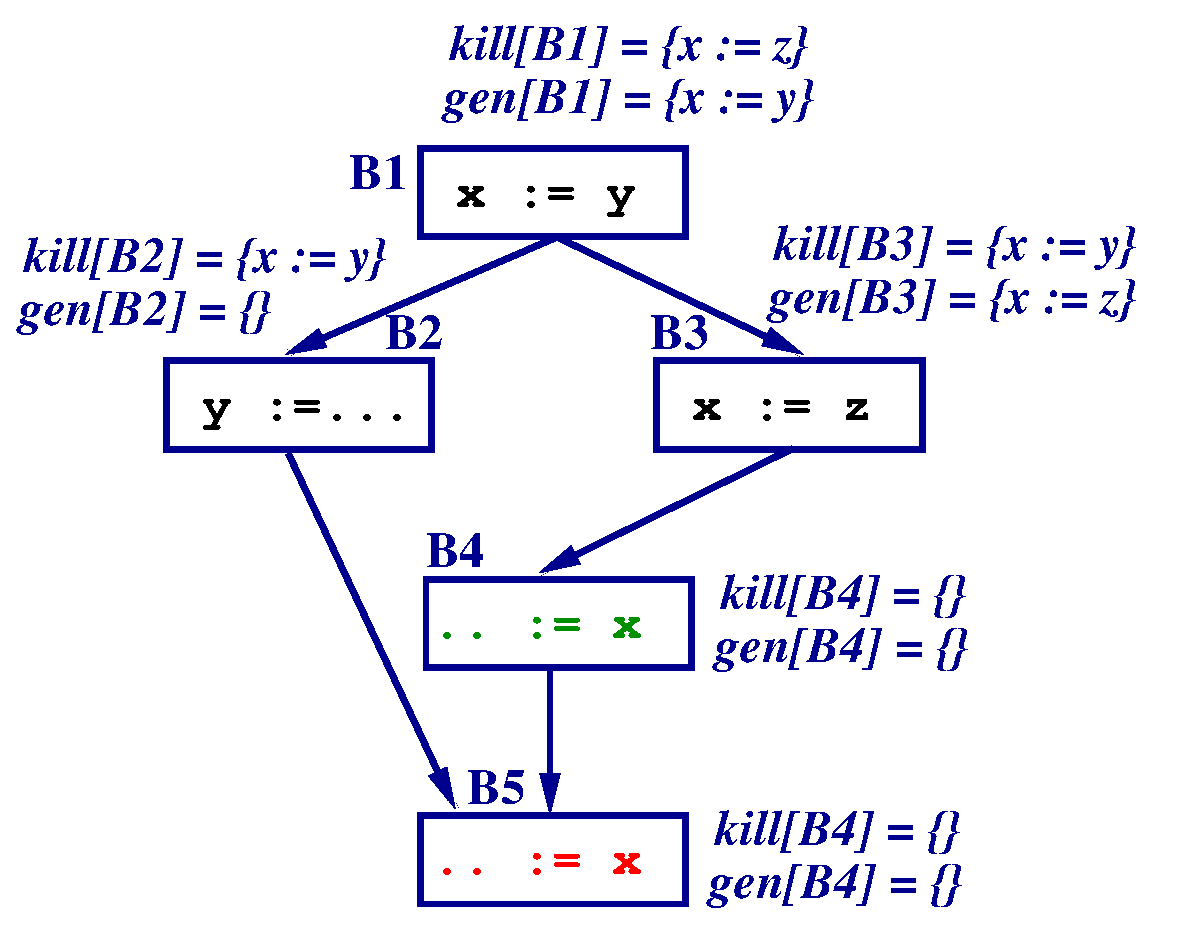
\includegraphics[width=44ex]{Figures/CopyProp}
\end{columns}
\end{block}

\end{frame}



\begin{frame}[fragile,t]
    \frametitle{Global Copy Propagation Algorithm}

\bigskip

\emph{\bf Algorithm.} For each copy stmt $\gamma$, of shape \blue{b := c} in program do:


\bigskip

\begin{itemize}
    \item Find all uses of \blue{\tt b} that are reached by $\gamma$, i.e., references to \blue{\tt b} in
            block $B$ such that $\gamma\in in_r[B]$ and $B$ does not contain any earlier
            redefinition of \blue{\tt b} or \blue{\tt c},\smallskip

    \item For each such use, if furthermore $\gamma \in in_c[B]$ then replace \blue{\tt b} by \blue{\tt c},\smallskip

    \item If replacement succeeds in all the above cases, then remove $\gamma$.
\end{itemize}

\end{frame}



\begin{frame}[fragile,t]
    \frametitle{Demonstrating Copy Propagation}


\begin{block}{Copy-Propagation Example}
\begin{columns}
\column{0.52\textwidth}
\includegraphics[width=37ex]{Figures/LoopCP}
\column{0.45\textwidth}
\emp{Copy stmt $1\in in_r[B_3]$ and
$1\in in_r[B_4]$. However 
$1\not\in in_c[B_3]$ and $1\not\in in_c[B_4]$,
hence replacement fails!}\\
$\mbox{~}$\\
\emp{Similar for copy stmt $2$.}\\
$\mbox{~}$\\
\blue{Copy stmt $3\in in_r[B_5]\cap in_c[B_5]$
and reaches the reference of {\tt n} in stmt $10$.}\\
\blue{Hence it is safe to delete stmt
$3$ and to replace {\tt n} with {\tt 10} in
stmt $10$!}
\end{columns}
\end{block}

\end{frame}

%%%%%%%%%%%%%%%%%%%%%%%%%%%%%%%%%%%%%%%%%%%%%%%%%%%%%%%%%%%%%%%%%%%%%%
\subsection{Common-Subexpression Elimination (CSE)}

%\begin{frame}[fragile]
%	\tableofcontents[currentsection]
%\end{frame}

\begin{frame}[fragile,t]
    \frametitle{Common-Subexpression Elimination (CSE)}

\emp{We wish to find two expressions that would always yield the same
        value, and to replace the second one with the result of the first!}

\bigskip

We say that \blue{\tt b op c} is an available expression at stmt $S$ iff:\smallskip
\begin{itemize}
    \item all routes from the start of the program to $S$ must pass through
            the evaluation of \blue{\tt b op c}, and\smallskip

    \item after the \emp{\bf last} eval of \blue{\tt b op c} there are no 
            redefinitions of \blue{\tt b} or \blue{\tt c}.
\end{itemize}

\pause
\bigskip

\emph{This means that in $S$ we can replace \blue{\tt b op c} with the result 
of its previous evaluation. {\bf Looks very similar to Copy Propagation!}}

\bigskip

Intuitively, we can think again of killing and generating expressions:\smallskip

\begin{itemize}
    \item \blue{b op c} is generated by the statement where it is evaluated,\smallskip

    \item \blue{b op c} is killed by a statement that redefines \blue{\tt b} or \blue{\tt c}.
\end{itemize}

\end{frame}



\begin{frame}[fragile,t]
    \frametitle{CSE at Basic-Block and Global Level}

\emph{\bf Basic-Block (B) Level}: Initially set $gen_e[B] = \emptyset$, then\smallskip

\begin{itemize}
    \item Go through $B$'s stmts in sequence, and for each \blue{\tt a := b op c}
        \begin{itemize}
            \item add \blue{\tt b op c} to $gen_e[B]$\smallskip
            \item delete any expression containing \blue{\tt a} from $gen_e[B]$\smallskip
        \end{itemize}
    \item $kill_e[B] =$ the set of all expressions anywhere in the program that
            are killed in $B$ by a redefinition of expression's operands.
\end{itemize}

\bigskip

\emph{\bf Init}: $in_e[B_1] = \emptyset$, $out_e[B_1] = gen_e[B_1]$, $out_e[B_i] = E - kill_e[B_i]$,
where $E$ is the set of all available expressions in the program.

\bigskip

\emph{\bf Data-Flow Equations}: for each basic block $B_i$, with $i \not= 1$:\smallskip

\begin{itemize}
    \item $in_e[B_i] = \cap_{B_j\in pred(B_i)}(out_e[B_j])$,\smallskip

    \item $out_e[B_i] = (in_e[B_i] - kill_e[B_i]) \cup gen_e[B_i]$.
\end{itemize}

\end{frame}




\begin{frame}[fragile,t]
    \frametitle{CSE Algorithm}

\bigskip

For each basic block $B$ do:

\bigskip

\begin{description}

    \item[(1)] Find all statements $\gamma$ of shape \blue{\tt a := b op c} 
                    in $B$, such that \blue{\tt b op c} $\in in_e[B]$, and $B$ 
                    contains no earlier definitions of \blue{\tt b} or \blue{\tt c}.\bigskip

    \item[(2)] For each stmt $\gamma$ found in \emph{(1)}, allocate fresh temporary \blue{\tt t}.\bigskip

    \item[(3)] From $B$, search backwards along all possible paths all
                    previous statements \blue{\tt d := b op c}, and immediately
                    after them insert \emp{\tt t := d}.\bigskip

    \item[(4)] Replace statement $\gamma$ by \emp{\tt a := t}.

\end{description}

\end{frame}



\begin{frame}[fragile,t]
    \frametitle{Demonstrating CSE}


\begin{block}{Common-Subexpression-Elimination Example}
\begin{columns}
\column{0.52\textwidth}
\includegraphics[width=37ex]{Figures/LoopCSE1}
\column{0.45\textwidth}
Only stmt $12$, i.e., \blue{\tt t4 := a-b} is
found in stage \emph{(1)} of Alg.\\
$\mbox{~}$\\
Searching backwards, the
unique previous evaluation is
in stmt $4$, hence insert 
\blue{\tt t5 := t1} as stmt $4$'.\\
$\mbox{~}$\\
Stage \emph{(4)} of Alg replaces 
stmt $12$ by \blue{\tt t4 := t5}\\
$\mbox{~}$\\
Subsequent copy propagation
and dead-code elimination will
eliminate \blue{\tt t4} and \blue{\tt t5}, 
i.e., both will be replaced by \blue{\tt t1}!
\end{columns}
\end{block}

\end{frame}


%%%%%%%%%%%%%%%%%%%%%%%%%%%%%%%%%%%%%%%%%%%%%%%%%%%%%%%%%%%%%%%%%%%%%%
%%%%%%%%%%%%%%%%%%%%%%%%%%%%%%%%%%%%%%%%%%%%%%%%%%%%%%%%%%%%%%%%%%%%%%


\end{document}
